\documentclass[10pt]{article}
\usepackage[usenames]{color} %used for font color
\usepackage{amssymb} %maths
\usepackage{amsmath} %maths
\usepackage[utf8]{inputenc} %useful to type directly diacritic characters
\usepackage{tikz}
\usetikzlibrary{arrows,positioning,decorations.pathreplacing} \begin{document}
\[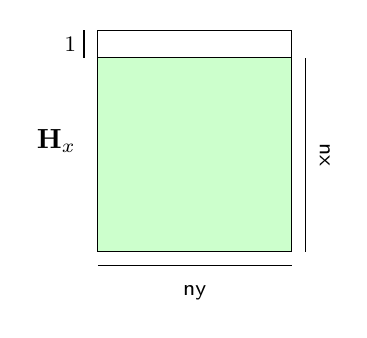
\begin{tikzpicture}
%
\node[draw=black,minimum width=7em,minimum height=8em,rectangle]  at (0,0) {};
\node[draw=black,fill=green!20,minimum width=7em,minimum height=7em,rectangle]  at (0,-0.5em) {};
%
\node[]  at (-5em,0) {${\bf H}_x$};
%
\draw[] (-4em,4em) -- (-4em,3em);
%\draw[] (-3.5em,4.5em) -- (-2.5em,4.5em);
\draw[] (-3.5em,-4.5em) -- (3.5em,-4.5em);
\draw[] (4em,-4em) -- (4em,3em);
%
\node[]  at (0,-5.5em) {\footnotesize{{\sf ny}}};
\node[rotate=-90]  at (4.7em,-0.5em) {\footnotesize{{\sf nx}}};
\node[]  at (-4.5em,3.5em) {\footnotesize{1}};
%\node[]  at (-3em,5em) {\footnotesize{1}};
\end{tikzpicture}
\]
\end{document}